\chapter{相关工作}
本文实验的系统,与信息抽取、本体学习等领域有较强的相关性,同时用到了自然语言处理、机器学习的一些模型和方法。下面对本文主要的相关工作作简单的介绍。
\section{信息抽取}

信息抽取(Information Extraction)是文本挖掘和信息检索中的一项重要任务,它的目标是从非结构化或半结构化的信息中发现结构化的特定信息,其中命名实体抽取,如人名、组织、地点,是最基础的任务,更复杂的抽取任务,如事件、关系抽取,依赖于精准的命名实体抽取。

信息抽取中早期的工作通常是基于规则的\cite{ciravegna2001adaptive}。首先,手工设计或者自动生成规则的集合,文本中的每个符号都被表示为特征的集合。一条规则包含一个正则表达式和动作。例如,一个识别人名的规则可能像这样:
\begin{center}
	(第一个词:``Mr.'',第二个词:首字母大写) $\rightarrow$ 人名
\end{center}
然后将文本和规则匹配,如果匹配成功,则执行对应的动作。如果有多条规则,需要定义规则执行的顺序,
例如顺序执行.

在特定的任务上基于规则的方法可以达到很好的性能,但是设计良好的抽取规则依赖于领域专家大量的工作,费时费力,并且针对一个目标的工作无法应用到其他目标中。因此,研究者之后将统计机器学习应用到信息抽取中,将信息抽取分解为不同的子问题,这些子问题可以转化为分类问题,可以使用支持向量机、最大熵模型等解决。信息抽取有时需要辨别文本的不同部分的语义角色,因此序列标注的方法被广泛应用。为了把实体抽取问题映射到序列标注问题,将句子中的每个词作为观察值,用BIO表示法标记文本块的边界。对每个实体类型T,类标B-T表示一个类型为T的实体名称开始,I-T表示位于T类型实体名称内部,O表示在任何一个名称外部,序列标注问题在于给出一个词序列,求出统计意义下最可能的标注序列。

\begin{problem}[序列标注]
已知观察值${\bf{x}} = ({x_1},{x_2}, \ldots {x_n})$,求最优序列标注${\bf{y^*}} = ({y_1},{y_2}, \ldots {y_n})$, 使得${{\bf{y}}^*} = \arg {\max _{\bf{y}}}P({\bf{y}}|{\bf{x}})$.
\end{problem}
在隐马尔科夫模型(HMM)中,对序列的生成过程做了马尔科夫假设,每个类标$y_i$仅由前一个类标$y_{i-1}$和$x_{i-1}$生成,每个观察值仅由该类标生成。转移概率可以在语料中进行频度估计,
\[
p(y_i=c|y_{i-1} = c, x_{i-1}=w) = \frac{n(c_1, c_2, w)}{n(c_2, w)}
\]
为了避免数据稀疏性的问题,可以加入必要的光滑。

HMM是一个生成模型,但数据较充足时,直接对$P(y|x)$进行建模的判别模型可能有更低的预测误差。\cite{mccallum2000maximum}将最大熵马尔科夫模型(MEMM)应用于信息抽取。在MEMM中,类标$y_i$依赖于附近的观察值$x_{i - l}^{i + l} = ({x_{i - l}},{x_{i - l + 1}}, \ldots ,{x_{i + l}})$和之前若干个类标

\begin{figure}[h]
\centering
\begin{subfigure}{0.3\textwidth}
\includegraphics[width=\textwidth]{HMM.png}
\caption{HMM}
\end{subfigure}
\qquad
\begin{subfigure}{0.3\textwidth}
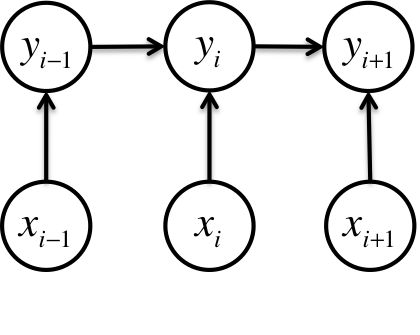
\includegraphics[width=\textwidth]{MEMM.png}
\caption{MEMM}
\end{subfigure}
\qquad
\begin{subfigure}{0.3\textwidth}
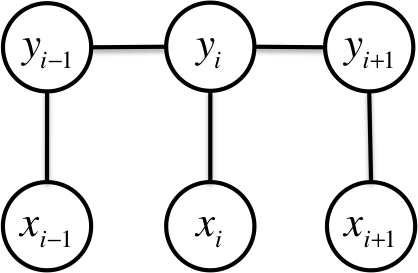
\includegraphics[width=\textwidth]{CRF.png}
\caption{CRF}
\end{subfigure}

\caption{序列标注模型}
\label{fig:seq_label_model}
\end{figure}


\section{本体学习}
本体学习(Ontology Learning)


\section{知识库}
知识库是对人类知识的结构化表示,它在搜索、智能系统中有着日益重要的应用,Google,Microsoft以及国内百度、搜狗等互联网企业均有自己的知识图谱计划。下面是常见知识库概况的一个总结。
\section{活动挖掘}
在活动挖掘方面,已有的工作非常有限。

\begin{table}[!h]
\begin{tabular}[0.7\textwidth]{|l|p{2cm}|l|p{4cm}|}
\hline
名称 & 开发者 & 概念数量  & 概述 \\
\hline
SenticNet & 南洋理工大学、新加坡国立大学 & 14,244	& 情感词汇  \\
\hline
Freebase & 社区	& 1450	& 对不同领域的知名人物、地点、事物 \\
\hline
WordNet\cite{miller1995wordnet} & 普林斯顿大学 & 25,229 & 英语词汇的知识库,根据同义语将英语词汇进行组织,并且提供词汇之间的多种语义关系。 \\
\hline
WikiTaxonomy\cite{ponzetto2007deriving}	& HITS & 127,325 & 基于维基百科(Wikipedia)的语料, 将类别按照is-a关系构建为一个大规模分类系统 \\
\hline
\end{tabular}
\caption{现有知识库概况}
\label{table:knowledge_base}
\end{table}

从表\ref{table:knowledge_base}中可以看到,现有的知识库种类繁多,但主要关注词汇,客观实体如人物、地点、物体的关系建模,没有对人类日常活动给予足够的关注。希望我的工作能在这方面对现有的知识库的一个补充。

\section{情感分析Sentiment Analysis}
我们希望了解用户参与
